\chapter{Information Visualization (infoVis)}

Human mind is very visual, following Williams et al., visualization is “a cognitive process performed by humans in forming a mental image of a domain space. In computer and information science it is, more specifically, the visual representation of a domain space using graphics, images, animated sequences, and sound augmentation to present the data, structure, and dynamic behavior of large, complex data sets that represent systems, events, processes, objects, and concepts”\cite{williamsVisualization1995}. The (Figure \ref{fig:roseDiagram}) below presents the Florence Nightingale's 'Rose diagram' published in 1858 showing the reduction in the number of deaths in military hospitals in Scutari arising from the changes she instituted\cite{spence2001information} .

\begin{figure}[h!]
    \center
    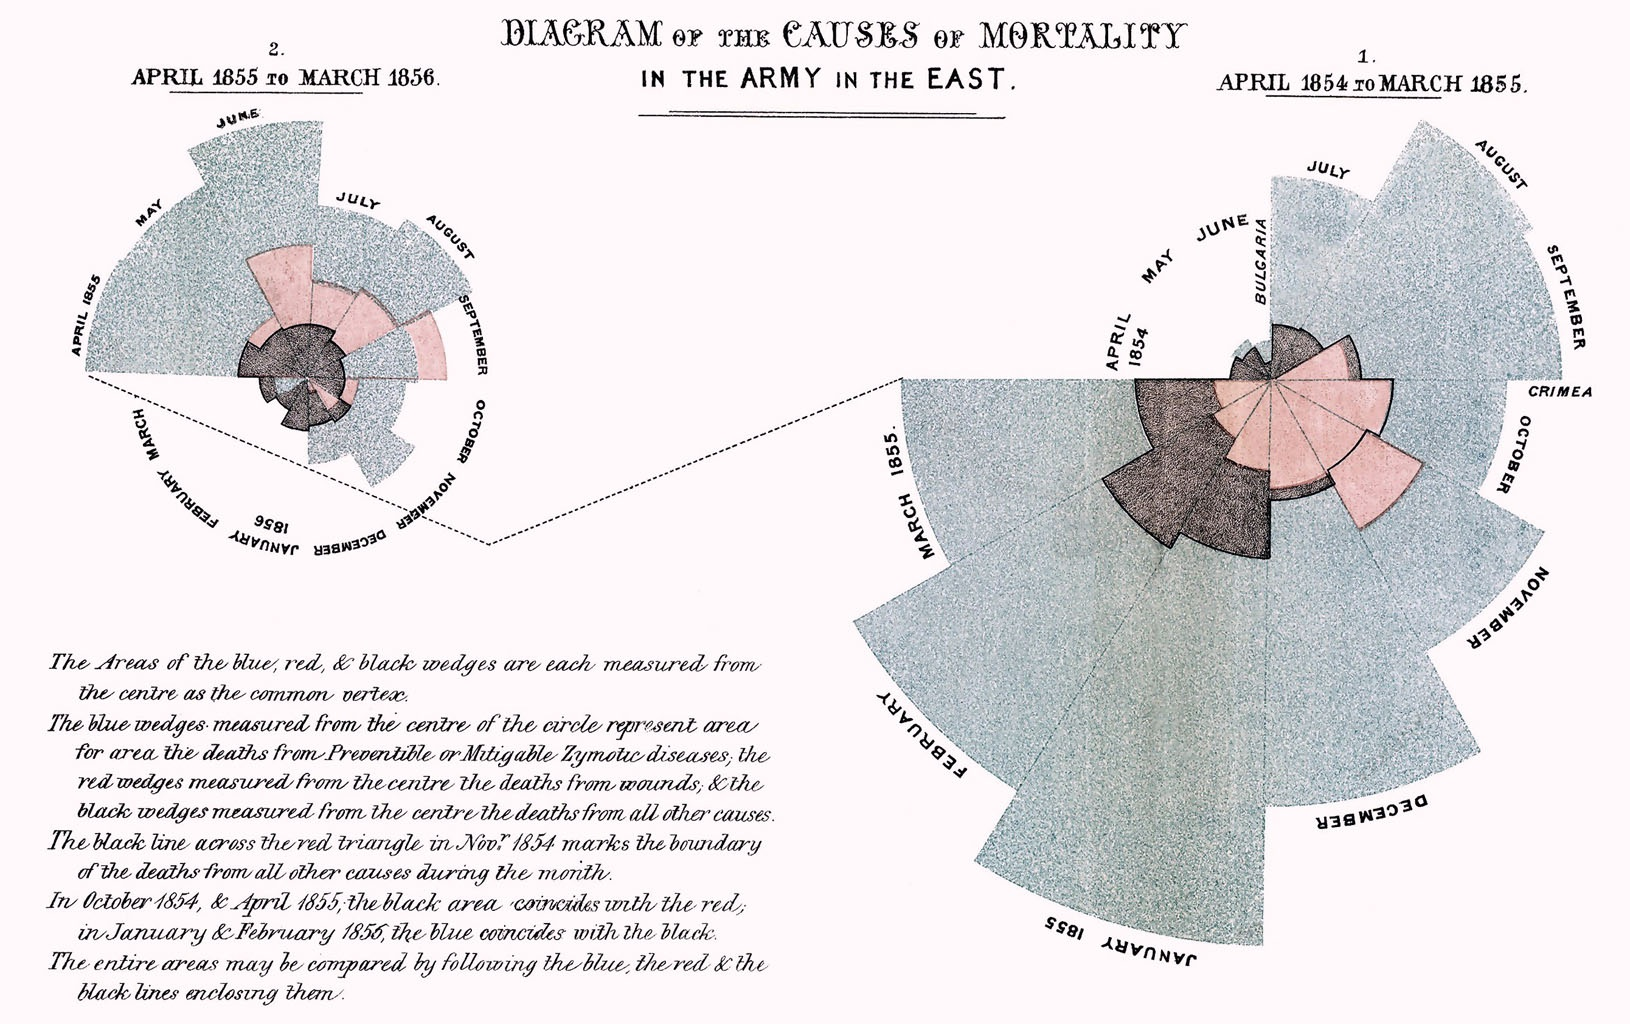
\includegraphics[width=0.78\textwidth]{images/chapter2/rose.jpg}
    \caption{Rose Diagram}
    \label{fig:roseDiagram}
  \end{figure}

 \newpage 
  Data visualization involves presenting data in graphical or pictorial form which makes the information easy to understand. It helps to explain facts and determine courses of action. It will benefit any field of study that requires innovative ways of presenting large, complex information\cite{spence2001information}.



  Traditionally, data visualization has been structured along two main fields: scientific visualization and information visualization. A third, newer field, called visual analytics has emerged in the past several years, as a bridge between and also an extension of the former two fields\cite{teleaDataVisualizationPrinciples2008}. In this paper we will focus mainly on the information visualization field.

\section{Definition}
Information visualization (InfoVis) is the practice of representing data in a meaningful, visual way that users can interpret and easily comprehend, it is a research area that aims to aid users in exploring, understanding, and analyzing data through progressive, iterative visual exploration. With the boom in big data analytics, InfoVis is being widely used in a variety of data analysis applications in different domains, ranging from finance to sports to politics\cite{liuSurveyInformationVisualization2014}.
\bigbreak
Information visualizations are often created with an audience in mind and designed to display certain important information that they need to understand. With an idea of how the visualization will be used, using multiple tools (Column chart, Bar graph, Network graph, Stacked bar graph, Histogram, Line chart, Pie chart, Box plot, Bubble chart,  Dual-axis chart,…)\ref{fig:infoViseType} that can help users compare different values, show the bigger picture, track trends in the data, and understand different relationships between variables\cite{WhatInformationVisualization}. These tools follow the model of the visualization pipeline. 

\begin{figure}[h!]
  \center
  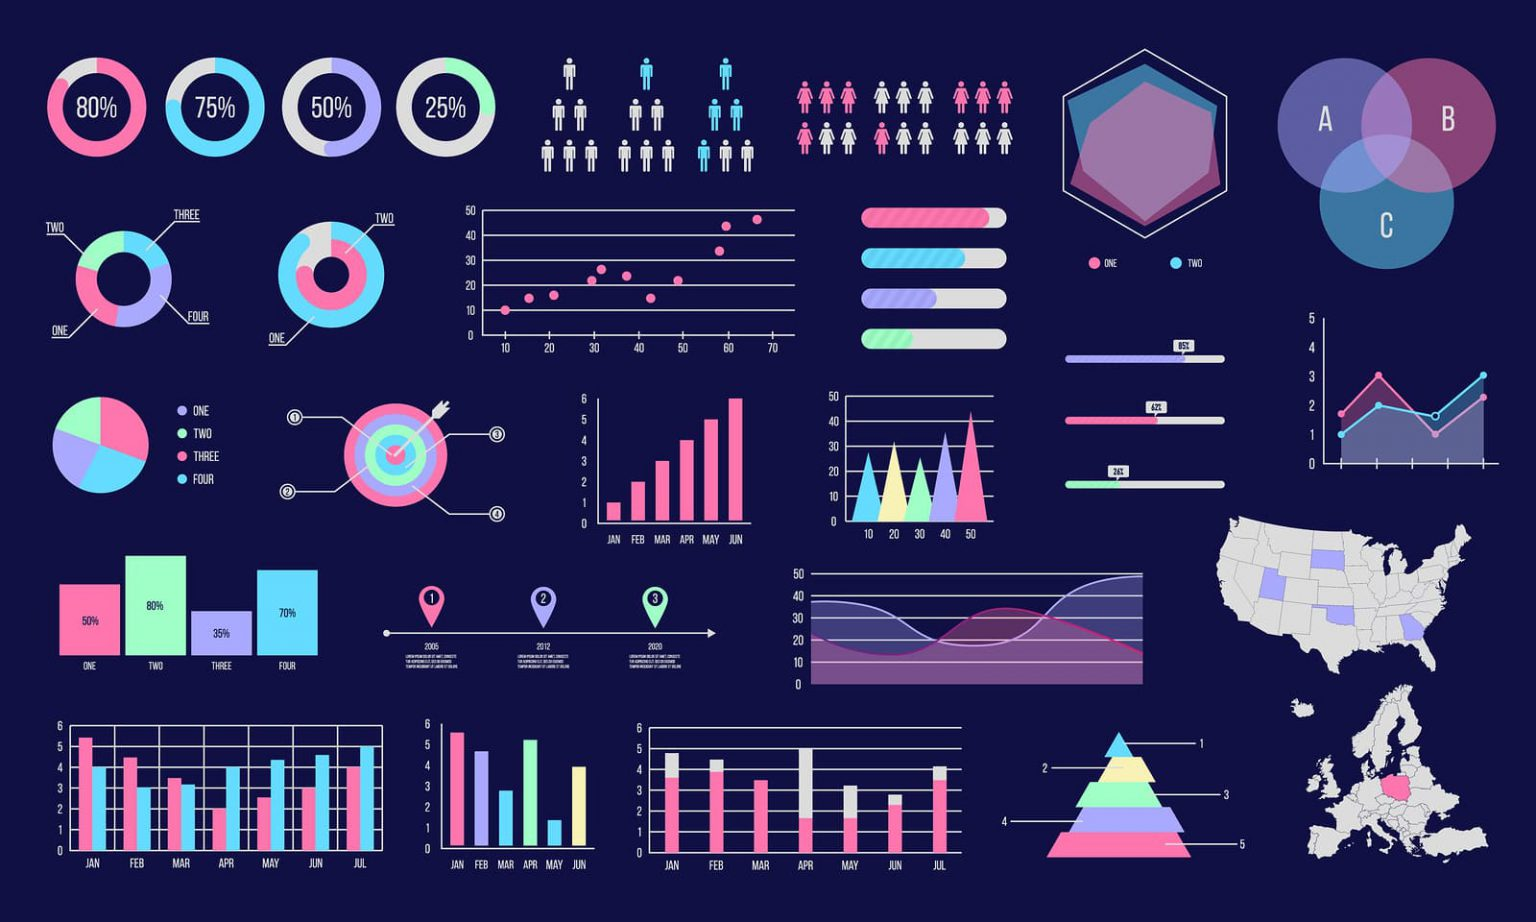
\includegraphics[width=0.60\textwidth]{images/chapter2/types-of-data-visualization.jpg}
  \caption{Information visualization tools}
  \label{fig:infoViseType}
\end{figure}

\section{Visualization pipeline}
\label{sec:visualization_pipeline}
A visualization pipeline embodies a dataflow network in which computation is described as a collection of executable modules that are connected in a directed graph representing how data moves between modules. In a \underline{basic} pipeline (Figure \ref{fig:simplepipeline}), there are three types of modules: sources, filters, and sinks. A source module produces data that it makes available through an output. File readers and synthetic data generators are typical source modules. A sink module accepts data through an input and performs an operation with no further result (as far as the pipeline is concerned). Typical sinks are file writers and rendering modules that provide images to a user interface. A filter module has at least one input from which it transforms data and provides results through at least one output\cite{morelandSurveyVisualizationPipelines2013}.

\begin{figure}[h!]
  \center
  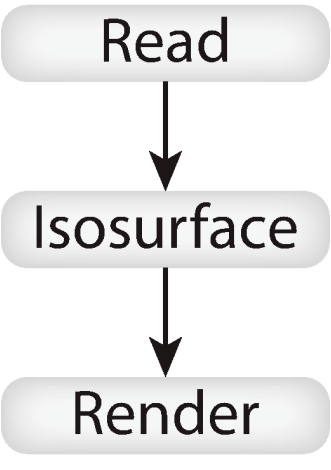
\includegraphics[width=0.20\textwidth]{images/chapter2/simplepipline.PNG}
  \caption{A simple visualization pipeline.}
  \label{fig:simplepipeline}
\end{figure}

\bigbreak
As science progresses, this model has been detailed, Figure \ref{fig:infovispipeline} provides an overview of the infoVis pipeline. It has five main modules: Data Analysis, Filtering, Mapping, Rendering, Image data, explained as follows:


\begin{figure}[h!]
  \center
  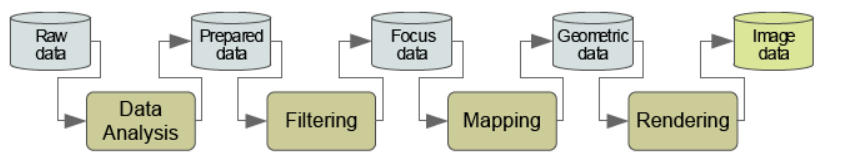
\includegraphics[width=0.80\textwidth]{images/chapter2/infoVispipeline.PNG}
  \caption{A visualization pipeline describes the process of creating visual representations of data.}
  \label{fig:infovispipeline}
\end{figure}


 
\begin{enumerate}
  \item \textbf{\textit{Raw data:}} First, we have to import the data. This implies finding a representation of the original information we want to investigate in terms of a data set. Practically, importing data means choosing a specific dataset implementation and converting the original information to the representation implied by the chosen dataset in order to turn this data into information using Data analysis.
  \item \textbf{\textit{Data Analysis:}} Is the process of bringing order and structure to collected data. mostly using data warehouse systems (\ref{sec:dataWarehouse}), It turns data into information  that teams can use. Analysis is done using systematic methods to look for trends, groupings, or other relationships between different types of data\cite{DataAnalysisVisualization}, following this process:
  \begin{itemize}
  \item \textbf{\textit{Data Requirements Specification:}} The data required for analysis is based on a question or an experiment. Based on the requirements of those directing the analysis, the data necessary as inputs to the analysis is identified (e.g., Population of people). Specific variables regarding a population (e.g., Age and Income) may be specified and obtained. Data may be numerical or categorical\cite{DataAnalysisProcess}.
  \item \textbf{\textit{Data Collection:}} Guided by the requirements identified, Data can be collected through several sources, including online sources, computers, personnel, and sources from the community.
  \item \textbf{\textit{Data processing:}} The data that is collected must be processed or organized for analysis. For instance, these may involve placing data into rows and columns in a table format (known as structured data) for further analysis, often through the use of spreadsheet or statistical software\cite{DataAnalysis2022}.
  \item \textbf{\textit{Data Cleaning:}} The processed and organized data may be incomplete, contain duplicates, or contain errors. Data Cleaning is the process of preventing and correcting these errors\cite{DataAnalysisProcess}. 
  % TODO: correct this link : https://www.tutorialspoint.com/excel_data_analysis/data_analysis_process.htm#:~:text=Data%20Analysis%20is%20a%20process,%2C%20and%20supporting%20decision%2Dmaking.
  \item \textbf{\textit{Perform data analysis:}}  One of the last steps in the data analysis process is analyzing and manipulating the data. This can be done in a variety of ways depending on the cleaned data nature\cite{WhatDataAnalysis}.
  \end{itemize}
  The data analysis step produces the \underline{prepared data}.
  \item \textbf{\textit{Filtering:}} Data filtering is the process of choosing a smaller part of your data set and using that subset for viewing or analysis\cite{WhatDataFiltering}, this portion of data called \underline{focus data}. 
  \item \textbf{\textit{Mapping:}} Focus data are mapped to geometric primitives (e.g., points, lines) and their attributes (e.g., color, position, size); most critical step for achieving expressiveness and effectiveness.
  \item \textbf{\textit{Rendering:}} The rendering operation is the final step of the visualization process, rendering takes the geometric data created by the mapping operation and transforms it to an image data.
  \end{enumerate}
  



\section{Data Warehouse Systems}
\label{sec:dataWarehouse}
The concept of "data warehousing" arose in the mid 1980s with the intention to support huge information analysis and management reporting\cite{wahDevelopmentDataWarehouse2009}. Data warehouse was defined According to Bill Inmon a “subject-oriented, integrated, time variant and non-volatile collection of data in support of management’s decision making process”\cite{inmonBuildingDataWarehouse2005}.
 
 
According to Ralph Kimball "a data warehouse is a system that extracts, cleans, conforms, and delivers source data into a dimensional data store and then supports and implements querying and analysis for the purpose of decision making"\cite{kimballDataWarehouseETLToolkit2011}.

There are three major areas in the data warehouse architecture as following:
\begin{itemize}
  \item \textbf{\textit{Data Acquisition:}} This step covers the process of extracting data from the multi sources, moving all extracted data to the stage and preparing the data for loading into the repository. The two main architectural components of this area are the source data and the data store, which is where all the extracted data is gathered and prepared for loading into the data warehouse.
  
  Following the medical data that are mentioned in the Table\ref{tab:sourceTable}, we chose to work on  the 3 different data related to different medical actors:

  
  %TODO: re check les termes ta3 les data qui vont etre visualizer
  \underline{Administrative} data, data relating to \underline{medical procedures} and data relating to \underline{the drugs administered to the patient} that are explained in chapter\ref{chap:healthData}.
  \item \textbf{\textit{Data processing and storage:}} This stage covers all preparations and analysis that take place on our data from data cleaning to data processing to filtering till the rendering step (the steps mentioned in section\ref{sec:visualization_pipeline}).
  At this stage, the data goes through a series of transformations to extract the focus data into clear and clean formats to build a sort of common language.

  \item \textbf{\textit{Information visualization:}} This step focuses mainly on the visualization part, it makes it easy for the users to access the information directly from the data warehouse.
\end{itemize}



\newpage
\section{Data Integration Approaches} 
Data integration is the most tedious and time-consuming step in setting up a decision-making information system. During this step, the data is transformed and filtered to represent a homogeneous, common and stable source of information. The performance of the SID is closely linked to the quality of data integration. It should be noted that the data integration step is not limited to the decision-making domain. It is more general and can be applied for different needs: bringing together and requesting several operational information systems, communicating applications that have been made in silos (independently of each other), etc.
 
Several approaches have been developed depending on the integration needs. We present the most used approaches\cite{naitEntropot}:
\begin{itemize}
  \item \textbf{\textit{Extract Transform and Load (ETL):}}\newline This is the most used approach in setting up a data warehouse. In this approach, the integration is done in three steps:
\begin{itemize}
\item Extracting data from sources.
\item Data transformation, which consists of cleaning and aggregating data to integrate them into a predefined schema.
\item Loading data into the target (the data warehouse).
\end{itemize}

  \item \textbf{\textit{Enterprise Information Integration(EII):}}\newline In the EII approach, no physical integration is performed. Heterogeneous data sources are consolidated using a virtual database, transparent to applications using the data. The virtual database provides a unified view of data. Users send their request directly to the database. The query is then broken down into sub-queries that will be sent to the respective sources. The answers are assembled into a final result.
  \item \textbf{\textit{Enterprise Application Integration(EAI):}}\newline In order to connect applications built in different environments and with different technologies, the EAI approach is based on application integration and sharing of their data using web services (SOA architecture). This approach allows for real-time communication.
It is also used to feed data warehouses. This approach does not replace ETL.
\end{itemize}

\begin{table}[h!]
    \centering
    \begin{tabular}{|m{0.25\linewidth}||m{0.25\linewidth}|m{0.25\linewidth}|m{0.25\linewidth}|}
        \hline

        \textbf{Criteria}                             & \textbf{ETL}        & \textbf{EII}         & \textbf{EAI}                  \\

        \hline
        Data flow 	& Unidirectional	& Bidirectional		& Bidirectional     \\
        
        \hline
        Latency	    & Daily to monthly	& Real time	    & Real time       \\
        
        \hline
        Data transformation	    & Big capacity		& Medium capacity	& Low capacity        \\
        
        \hline
        Context of use	    & -Consolidation of a large amount of data.\newline -Complex transformations.	    & -Link an existing warehouse with specific data sources.\newline -Source data volatile and accessible using simple queries.    & -Sources not directly accessible.\newline -Simple queries.       \\
        
                
        \hline
    \end{tabular} 

    \caption{Comparison between different integration approaches.}
    \label{tab:approaches}
\end{table}
